\documentclass[a4paper,11pt,titlepage]{scrbook}

\usepackage{graphicx}
\usepackage{fancyhdr}         % Define simple headings
\usepackage{vmargin}          % Adjust margins in a simple way
\usepackage{tikz}
\usepackage{polyglossia}
\setdefaultlanguage{english}
\usepackage{booktabs,makecell}
\usepackage[binary-units=true]{siunitx}
\usepackage[autopunct=true]{csquotes}
\renewcommand{\mktextquote}[6]{#1#2#4#5#3#6}
\usepackage[labelfont=bf,format=plain]{caption}
\usepackage{enumitem}
\setlist{itemsep=0.3ex}
\setlist[enumerate]{label = (\alph*)}
\usepackage[backend=biber,style=alphabetic]{biblatex}
\usepackage{amssymb}
\usepackage{mathtools}
\usepackage{pgfplots}
\pgfplotscreateplotcyclelist{mylist}{%
    draw={rgb,1:red,0.368417;green,0.506779;blue,0.709798},thick\\%
    draw={rgb,1:red,0.880722;green,0.611041;blue,0.142051},thick\\%
    draw={rgb,1:red,0.560181;green,0.691569;blue,0.194885},thick\\%
    draw={rgb,1:red,0.922526;green,0.385626;blue,0.209179},thick\\%
    draw={rgb,1:red,0.528488;green,0.470624;blue,0.701351},thick\\%
}

\addtokomafont{disposition}{\rmfamily}
\renewcommand*{\headfont}{\slshape}
\newcommand{\blankpage}{
 \clearpage{\pagestyle{empty}\cleardoublepage}
}
\setcounter{secnumdepth}{3}
\setcounter{tocdepth}{3}

\pagestyle{fancy}
\renewcommand{\chaptermark}[1]{\markboth{\thechapter.\ #1}{}}
\fancyhf{}
\fancyhead[LE,RO]{{\headfont\thepage}}						% Left/right header for even/odd pages
\fancyhead[LO]{\headfont\nouppercase{\rightmark}}	% Header for left page (odd)
\fancyhead[RE]{\headfont\nouppercase{\leftmark}}	% Header for right page (even)
\fancyfoot[C]{\thepage}
\renewcommand{\headrulewidth}{0.5pt}
\renewcommand{\footrulewidth}{0pt}
\fancypagestyle{plain}{%
\fancyhf{}													% No Header and Footer fields
\renewcommand{\headrulewidth}{0pt}
\renewcommand{\footrulewidth}{0pt}
\fancyfoot[C]{\thepage}
}

\widowpenalty 10000
\clubpenalty 10000


\begin{document}


\frontmatter
\pagenumbering{roman}
\chapter*{Abstract}
% TODO
\dots

\tableofcontents
\blankpage

\mainmatter
\pagenumbering{arabic}
\chapter{Introduction}

% As was outlined in the introduction, deliberate inclusion of problematic data into the Blockchain, such as copyright-protected, illegal, or politically sensitive content, could render the possession of the Blockchain illegal in most jurisdictions.
% Hence, due to persistency of the blockchain, this malicious inclusion harms every participant in Bitcoin's network, and might make participation even legally impossible.

\chapter{Data inclusion in the blockchain}

This section describes the state-of-the-art method how the transaction structure of the Bitcoin blockchain enables the inclusion of arbitrary data in the blockchain.
For this, we first outline the transaction processing of the Bitcoin network on the basis on its scripting language. Then, describe the techniques how this structure can be exploited for data inclusion, and sensibly restrict our considerations on one specific technique type.


\section{Transaction structure and processing}

%In essence, the Bitcoin network defines its corresponding \textquote{electronic coin as a chain of digital signatures.
%ach owner transfers the coin to thenext by digitally signing a hash of the previous transaction and the public key of the next owner and adding these to the end of the coin.}

In the Bitcoin network, transfer of electronic coins is realized using \emph{transactions}.
From a structural perspective, every transaction specifies a set of \emph{transaction input} and a set of \emph{transaction outputs}, with every input referencing a previous transaction's output.
Following these references, each transaction can be considered the root of a directed acyclic graph, where transactions are considered vertices, and its references the directed edges.

In order to give this transaction authenticity, an elligible user attaches to each reference some form of digital signature.
By verifying each signature associated to the preceding transactions in the graph, one can follow and verify the chain of ownership of the coins.
Hence, strictly speaking, \textquote*{ownership of coins} in the Bitcoin network is the ability to create a transaction referencing outputs not already references, using ownership of private keys in oder to generate valid signatures.

Bitcoin implements the authenticity system of these references using a challenge–response authentication between the referenced transaction outputs and the transaction inputs.

\begin{itemize}
    \item Every output contains a \emph{locking script}, which can be understood as the cryptographic puzzle or challenge, which was defined when the transaction was constructed.
        %E.g.\@ a public key of the person owning this transaction.
    \item An reference to a output from an input is authentic, if the corresponding \emph{unlocking script} can solve the challenge imposed by the referenced output.
        %E.g.\@ a signature of the transaction referencing the output, generated by the private key matching the corresponding public key embedded in the input.
\end{itemize}

Bitcoin provides several methods for implementing locking and unlocking scripts, and as example, the widespread pay-to-public-key script types are presented: In this scenario, a payee Bob expects the payer Alice to publish a transaction with his public key embedded in the locking script of an output $x$.
Then, to transfer these coins to Charlie, Bob constructs a transaction $t$ with an input referencing $x$, adding to the unlocking script a signature of message $t$, signed with his private key, corresponding to the public key embedded in $x$.
Then Bob can add the output with the locking script expected by Charlie, and submit the transaction.


The network verifies this reference by checking the signature of the unlocking script against the public key embedded in the locking script.


Implementation-specific, Bitcoin employs a \emph{Elliptic Curve Digital Signature Algorithm} (using parameters from SEC2-secpk256k1) as public-key system.
Henceforth, we refer to $G\in \mathbb{F}_p^2$ as the base point of the elliptic curve group (over the finite field of prime order $p$). For $x\in \mathbb{N}$, let $x\cdot G$ denote the elliptic curve point multiplication by a scalar.

Following table summarizes the five standard locking script types (i.e.\@ address types) with their corresponding unlocking script. Any other forms of locking scripts are currently being rejected by network participants.Hash function $H$ is implemented in Bitcoin as composition of first SHA256, followed by RIPEMD160.

\begin{table}
    \renewcommand{\arraystretch}{1.2}
    \centering
    \begin{tabular}{lll}
        \toprule
        \textbf{Type} & \textbf{locking script\,/\,address} & \textbf{unlocking script} \\
        \midrule
        P2PK & pubkey $x\cdot G$ & sig of tx with $x$ \\
        P2PKH & hash of public key $H(x\cdot G)$ & $x\cdot G$, sig of tx with $x$ \\
        P2MS & pubkeys $x_1{\cdot} G, x_2{\cdot} G, \dots, x_n{\cdot} G$ & sigs of tx with $x_{i_1}, \dots, x_{i_m}$ \\
        P2SH & hash $H(s)$ of redeem script $s$ & $s$ plus additional data $y$ \\
        Null Data & $\leq \SI{80}{\byte}$ arbitray data & (unspendable)\\
        %P2SH* & $x\in [0{:}2^{160}]$ & $H(x)$ \\
        \bottomrule
    \end{tabular}
    \caption[Overview of the discussed standard address types]{Overview of the discussed standard address types: P2PK (pay-to-public-key), P2PKH (pay-to-public-key-hash), P2MS (pay-to-multisig), P2SH (pay-to-script-hash), Null Data. For pay-to-multisig (P2MS), $1\leq m\leq n\leq 3$ is required to be considered standard. See following text for a definition of redeem script.}
\end{table}

The P2SH (pay-to-script-hash) type requires further explanation: this address type is a generalization of the challenge–response authentication employed by the network, and allow users to create their own challenges and responses using a limited scripting language.
A locking script consists of the hash of the challenge script $s$ (called \emph{redeem script}), while the unlocking script must contain the corresponding redeem script (transfered off-band to the payee), and additional parameters $y$ that the author of the redeem script $s$ requires as input to $s$ to be processed, checking authenticity of the payee.




\section{Script-based data inclusion}

The Bitcoin network further employs a blockchain as a distributed data structure to prevent double-spending of transaction outputs, i.e.\@ multiple references to the same output.
The blockchain acts as timestamping mechanism, by providing \textquote{a system for participants to agree on a single history on the order \textins{of transactions} in which they were received}, hence storing every transaction with its relevant information in that data structure on time of submission.

This data structure disallows any modification on the agreed set of transaction \emph{by design}, 
as to maintain the chain of ownership induced by the transactions.
Hence the locking and unlocking scripts of every transaction are stored in the blockchain, essentially indefinitely.

\subsubsection*{Inclusion on outputs\,/\,locking scripts}

From this, the Null Data transactions already allow any user to create unspendable transactions that contain up to \SI{80}{\byte} of arbitrary data payload, yet are, due to the length limitation, costly and not suitable for large quantites of data.

Therefore, more sophisticated techniques for data inclusion build upon the fact, that the network does not, and cannot test if the variable parts of the locking scripts, e.g.\@ pubkey(s) $x\cdot G$ in P2PK/P2MS transactions, hashes $H(x\cdot G)$, $H(s)$ in P2PKH/P2SH transactions, are in fact, generated using the usual intended way.
For example, consider payload $y$ of \SI{65}{\byte}.
The network accepts and stores a P2PK transaction with $y$ as \textquote{fake} public key its locking script, even though $y\neq x\cdot G$ for all $x$ (in fact, even if $y$ does not conform the syntax of a EC point).
Again, this means that the coins \textquote*{sent} to the fake address $y$ cannot be spent, i.e.\@ \emph{burnt} coins, just as it is the case of Null Data transactions.
Unlike Null Data outputs, a multitude of P2PK output can be present in a transaction, making the technique using P2PK outputs more efficient.
Refer to the paper of Sward et al.\@ for an in-depth discussion of efficiencies using this technique.

\subsubsection*{Inclusion on inputs\,/\,unlocking scripts}
While the previously presented inclusion techniques insert their payload in the locking scripts, Sward et al.\@ analyzed inclusion approaches using P2SH unlocking scripts.
Again considering payload $y$, they construct a specialized redeem script $s$ and unlocking script $s'$, 
such that $y$ is a substring in $s'$.
To now perform the inclusion into the blockchain, first one publishes a transaction containing P2SH output with $H(s)$, then another transaction referencing this output, containing $s'$ as unlocking script.
This results in two valid transactions, and even require no burnt coints.
In fact, Sward et al. showed that this technique outperforms every known inclusion technique using locking scripts, given the fact that unlocking scripts have a much higher size limitation in comparison to locking scripts, which have a fixed format.

Nevertheless, we will exclude an analysis of this inclusion technique in this report.
These complex transaction types might be the easiest to ban or limit, if data inclusion using P2SH were to become a problem.
Since most P2SH transaction effectively implement a multisig scheme, a concensus for imposing a fixed structure for redeem scripts might be established quickly, especially if data inclusion using unlocking scripts causes major threats.



% ignore input-script-insertions <-> assume non-standard scripts banned
% P2SH-method uses non-standard script and is not suited for analysis(?)
% required unlocking input however provably is a  public key

% P2MS??


\chapter{Countermeasure and Circumvention}

%Many extensions are discussed that attempt to mitigate the problem of off-topic data inclusion, which, as was outlined in the introduction, can cause unwanted vulnerabilities to the Bitcoin blockchain.
%We focus on proof-of-ownership countermeasures, since that method appears to be the strongest while respecting the principles of the Bitcoin network (permissionless, irreversible, etc.) 
The following section first gives a detailed definition of the proof-of-ownership countermeasure. After specifying the functionality and demonstrating its intended effect, we develop an efficient brute-force method to circumvent this countermeasure. Last part of the section gives details on how to implement such circumvention in practice.

A straightforward idea for preventing data inclusion attempt to make the network \textquote*{forget} stored information after processing, or allow the network to remove undesirable data, or recognize bad transactions using a heuristic, before they are distributed and stored.
However, all these preventions conflict with certain properties of the network, that are universally considered characterizing for the Bitcoin system.
Hence, the adoption of such countermeasure would transform the Bitcoin system in such an extent, that the resulting a electronic cash system would in general not be considered \textquote*{Bitcoin}.

While there is no central authority stating these properties, the corresponding \emph{Bitcoin Wiki} text can serve as representative for the concensus of the community:
\begin{displayquote}
    \noindent
    \textooquote{}All changes and upgrades to the protocol should strive to maintain and reinforce these Principles of Bitcoin

    \begin{enumerate}[label={[}\arabic*.{]}]
        \item 21 million coins.
        \item No censorship: Nobody should be able to prevent valid txs from being confirmed.
        \item Open-Source: Bitcoin source code should always be open for anyone to read, modify, copy, share.
        \item Permissionless: No arbitrary gatekeepers should ever prevent anybody from being part of the network (user, node, miner, etc).
        \item Pseudonymous: No ID should be required to own, use Bitcoin.
        \item Fungible: All coins are equal and should be equally spendable.
        \item Irreversible Transactions: Confirmed blocks should be set in stone. Blockchain History should be immutable.\textcoquote
    \end{enumerate}
\end{displayquote}
The mentioned countermeasures above would contradict principles 4, 5, or 7, at least.

Hence we continue our analysis only on countermeasures that are compatible with these properties,
since all nonconforming countermeasures might face serious opposition to adoption from the community.
From these principles appear to follow, that these countermeasures must respect following propositions, when determining if a submitted transaction contains no bad data:
\begin{enumerate}
    \item The assessement needs to be made in a transparent way, especially without an authoritative figure (by principle 4),
    \item it needs to be made \emph{before} publication of the transaction (by principle 7).
    \item Every honest user can convince the countermeasure that its submitted transaction is not bad, without relying on third parties, i.e.\@ proof derivable from the private key only (by principle 2, 5, 6).
\end{enumerate}
As a consequence, an \textquote{honest participant} necessarily needs to be identified by \textquote{control of their private key}.
Hence a submitted destination address is clean if the owner of that address can prove control, that is, ownership of the address.

Following section introduces a Proof-of-ownership countermeasure that appears to be the strongest one respecting these propositions, motivating the evaluation of this countermeasure and its circumvention.


\section{Proof-of-ownership countermeasure}

In his Master's thesis \emph{Hardening Bitcoin against off-topic data inclusion}, Seeg proposes a countermeasure to this problem using a proof-of-ownership mechanism, which he calls \textquote{preimage solution}. 
%He observes that \textquote{variants that store data in standard transactions output can be mitigated by requiring proof that the variable parts}, that is, public keys (P2PK), public key hashes (P2PKH), script hashes (P2SH), \textquote{of the standard transactions are clean.}
%
He considers an address as clean (i.e.\@ without arbitrary data) if and only if the owner of that address can prove control, that is, ownership of the address.
Such proof of ownership is derived from the \textquote*{private} preimage part of the address, similar to a classic challenge–response authentication.
The wanted effect follows from the assumption that given \textquote*{public} part of a non-clean address, one cannot efficiently derive \textquote*{private} preimage required for the proof of ownership.

For P2PK address types, this translates into a proof using signatures, which certify the control of the corresponding private key.
That is, in order for Alice to send coins to Bob, he sends her off-band his public key $x\cdot G$, and a signature $\sigma$ verifying message $m=H(x\cdot G)$, generated using private key $x$.
Then, Alice can construct a P2PK transaction with recipient key/address $x\cdot G$, and when submitting the transaction to the network, she attaches $\sigma$ which proves that Bob indeed controls that address. 
(This entails that $\sigma$ needs to be transmitted off-band to Alice before the transaction.)
Miners can verify $\sigma$ using the public key $x\cdot G$ embedded in the transaction, approving the output address of the transaction.

This countermeasure protects against data inclusion: if an adversary wishes to embed message into public key $x\cdot G$, he cannot efficiently derive $x$, required in order to sign the proof $\sigma$.
Thus, given valid $\sigma$, the transaction in question can be safely included into the blockchain.

In the case of P2PKH and P2SH addresses, proofs are constructed in a similar manner.
For P2PKH addresses $H(x\cdot G)$, signed message $m$ remains identical.
Only the public key $x\cdot G$ is additionally transferred such that $\sigma$ can be verified by the network.
For P2SH addresses $H(s)$, the redeem script $s$ serves as preimage/proof $\sigma$.
Again, this prevents data inclusion due to the one-way property of hash function $H$.
(Note that in the case of P2PKH and P2SH transactions, Seeg proposed a slightly weaker approach, exploiting the choice of $H$ as composition of two hash methods, and using the first digest as $\sigma$.)

In fact, this type of countermeasure appears to be one one of the strongest compatible with the Principles of Bitcoin.
Addresses that withstand the proposed test are to be precisely the addresses that can be generated by honest participants of the network, who should not be penalized by any countermeasure.
%This further motivates an evaluation of the proposed countermeasure.
Additionally, other countermeasures that respect these mentioned principles build on top of the one-way property of the same cryptographic functions in a similar matter, e.g.\@ \textquote{self-verifying account identifiers} proposed by Matzutt et al.
Therefore, this countermeasure and the respective circumvention act as representative for all one-way-based approaches.

% \section{Commitment-based countermeasure}
% TODO Matzutt??

\section{Circumvention using partial preimages}

% Refer to similarities between Seegs proofs and Matzutts ICs

In essence, the proposed countermeasure builds upon preimage resistance of specific cryptographic one-way functions,
in order to embed identifiers into transactions, that are provably clean by proving existence of the preimage.
That is, for given function $f$, preimage $x$ cannot be efficiently derived from image $f(x)$, whereas only $f(x)$ is stored in the blockchain.
Attempts to embed $y=f(x)$ hence become computationally hard.
The countermeasures use the (presumed) one-way property of Bitcoin's hash function and elliptic curve multiplication.
Incidentally, they correspond to the exact function translating a private key $x$ into a public key resp.\@ address $f(x)$.
Refer to table \ref{} \dots % TODO

No matter the chosen function $f$, the trivial approach to find a preimage to value $y=f(x)$ is via \emph{brute force}: we test pairwise different preimage candidates $x_1, x_2, \dots$ until we find $x_i$ such that $f(x_i)=y$.
The preimage $x_i$ can then be used to generate suitable proofs for the image (e.g.\@ signatures $\sigma$).
Nevertheless, successfully executing such a preimage attack is highly unlikely – in fact, if that attack were possible, an adversary could gain control of the funds assigned to any public key (by inverting the public-key function $f$).

While a full preimage attack is out of reach, \emph{partial} preimage attacks are achievable nonetheless:
Given a prefix bit-length $n$, we define $x$ as \emph{partial preimage} of $y$ when $f(x)$ equals $y$ \emph{in the first $n$ leftmost (most significant) bits}, i.e.\@ $f(x)=y\|z$ where $z$ is an arbitrary suffix.

For uniformly chosen private key $x$, we can assume that the respective $n$-bit prefix of the public key $f(x)$ is again uniformly chosen from the range $[0{:}2^n]$.
By this, the success probability of a successful partial preimage attacks increases to $1/2^n$, which, after sufficiently many repetitions and sufficiently small $n$, leads to suitable partial preimage $x$; the corresponding public key $f(x)$ then contains the wanted payload $y$ as prefix.
In terms of the proposed countermeasure, one would continue by constructing transaction containing output address $f(x)$ and proof $\sigma$ from $x$.
Submitting both would then successfully circumvent the countermeasure and include $y$ into the blockchain.

While the notion of prefixes is clear in the case of hash digests involved in P2PKH and P2SH addresses, such prefix of a public key $x\cdot G = (a,b) \in \mathbb{F}_p^2$ involved in P2PK addresses is not necessarily obvious.
To be definite, we define the $n$-bit prefix of $x\cdot G$ as the $n$ most significant bits of first coordinate $a$ of that curve point. 
(From the perspective of the SEC-defined curve point representation used in Bitcoin, this corresponds to bits 9 to 264. In fact, first byte of the SEC representation is fixed.)


\section{Implementation}

\begin{figure}
    \centering
    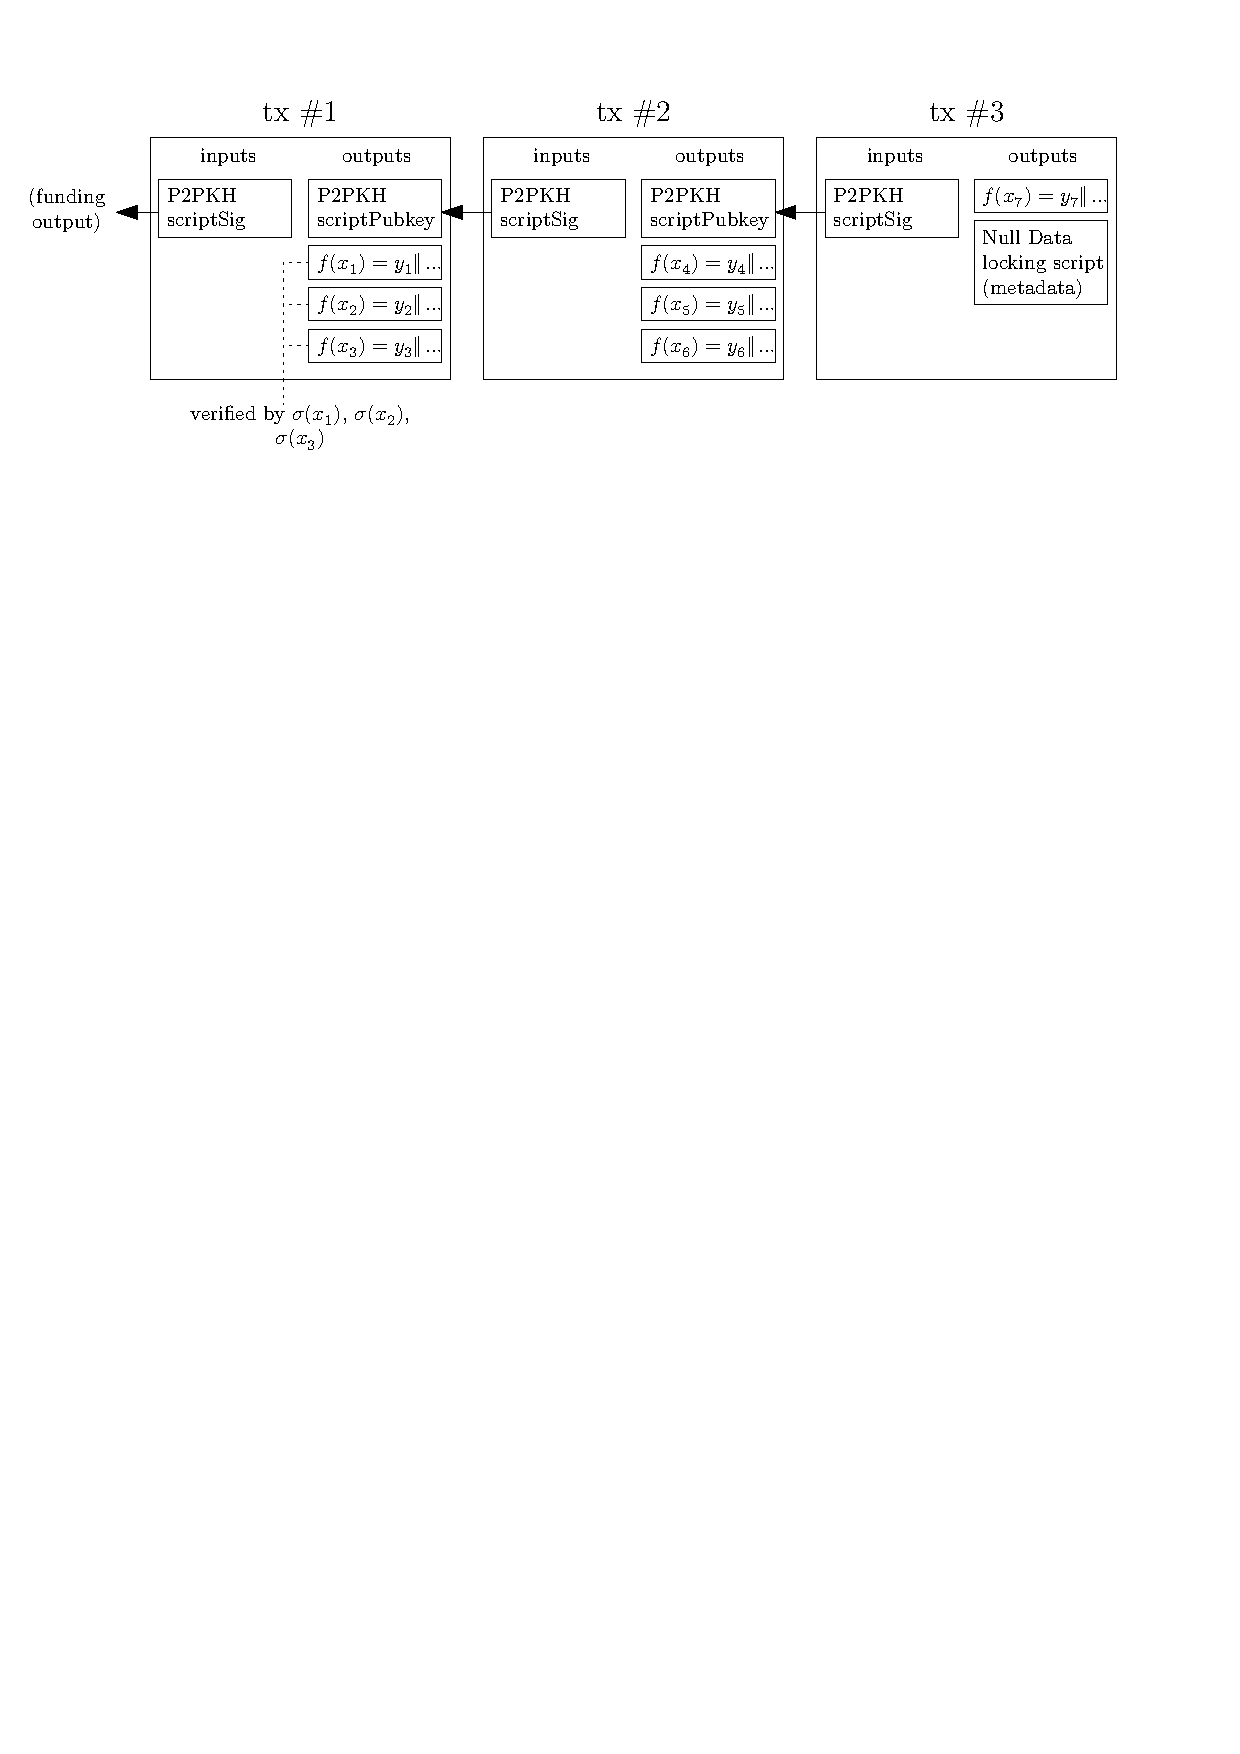
\includegraphics[width=14cm,keepaspectratio]{figure.pdf}
    \caption[Proposed scheme to construct transaction from the prepared addresses to circumvent the countermeasure]{Proposed scheme to construct transaction from the prepared addresses, which are partial preimages of the payload's fragments. Submitting tx \#1, \#2, \#3 together with the respective proofs $\sigma(x_1), \dots, \sigma(x_7)$ would then circumvent the countermeasure. Arrows from input to output signify which output the respective input is referencing; that is, the \emph{logical} direction is from right to left, the \emph{chronological} direction from left to right.}
    \label{fig:tx-construction}
\end{figure}

Having provided a framework showing the mathematical possibility to circumvent such countermeasure, following section describes the necessary steps to perform such inclusion in practice.
That is, including payload data in order into the blockchain, where the data is embedded into output addresses of transactions.
Additionally, following procedure generates private keys to each of the used output addresses, such that proofs of ownership can be deduced as required in the countermeasure, and hence the generated transactions are approved.
It is to be noted, that, in the context of Seeg's proposal, investing in a rainbow table could significantly increase performance in comparison to a full brute force approach.
Nevertheless we omit rainbow tables, since this issue could easily be solved when refining the countermeasure, e.g.\@ including transaction hash in the proof message $m$ to be signed.
Cf.\@ with the \textquote{freshness property} in Matzutt's approach.

The procedure is given with a chosen prefix length $n$. Performance and cost directly depend on this parameter, and a fit choice for $n$ is discussed in the next section.

\emph{Preparation.} First, we partition the payload into fragments $y_1, y_2, \dots, y_p$ of length $n$, and use a binary tree as efficient data structure to access the fragments, sorting them by their lexicographic order.

\emph{Partial preimage loop.} 
Then, we have to find a suitable partial preimage $x_i$ for every fragment $y_i$ with $1\leq i \leq p$ in the tree.
In each iteration (of the outer loop), we generate many private key candidates $x$ by brute force (inner loop), until the prefix of $f(x)$ matches any fragment remaining in the tree.
We then can assign matching fragment $y_i$ the private key $x_i \coloneqq x$.
This leads to a mapping $y_i \mapsto x_i$ for all $1\leq i\leq p$.

The implementation is trivial for the P2SH method: let $s$ be an injective function transferring a nonce $m$ into a valid redeem script.
We start off with a random nonce $m$, and test $H(s(m))$, increment $m$, test again, and so forth.
Having found $m$ with prefix of $H(s(m))$ matching one fragment in the tree, we can assign that fragment the private key $s(m)$.

In the case of the P2PK method, this translates to testing products $m\cdot G$, $(m{+}1)\cdot G$, $(m{+}2)\cdot G,\dots$ from random starting nonce $m$.
Using the axioms of the group formed by the elliptic curve, we can avoid costly elliptic curve multiplications: starting with random nonce $m$, we cache public key $P\coloneqq m\cdot G$.
When incrementing $m$, we add generator point to $P$, that is $P\coloneqq P+G$, and ensure invariant $P= m\cdot G$.
Again, having found $m$ with prefix of $P$ matching one fragment in the tree, we assign that fragment private key $m$.
The P2PKH method can be implemented similarly, by testing hashes $H(P)$.

\emph{Transaction construction.}
From assigned private keys, we can construct transactions containing the respective public keys $f(x_1), f(x_2), \dots$ in order, embedding the prefixes $y_1, y_2, \dots$.
That is, we construct a transaction with a single funding input, and add corresponding outputs containing the public keys as destination addresses, whereas every output must send a value of at least the non-dust amount of 546 sat.
If the size of the transaction exceeds a defined limit (or the network limit of $\SI{100}{\kilo\byte}$), we add an output referred by the next transaction as funding input, as depicted in figure \ref{fig:tx-construction}.
A terminal OP\_RETURN-output allows embedding of metadata, facilitating reconstruction of the data.
Since we have chained the transactions using funding inputs, the transaction identifier of the last transaction can serve as locator for the data in the blockchain.
It is recommended to use P2PK(H) scripts as funding inputs, since the signatures in the scriptSig parts effectively prevents modifications to the transaction, for example an unwanted reordering of the transaction outputs.

\emph{Signature generation and submission.}
Again, having the private keys $x_1, x_2, \dots$, it is trivial to generate the proofs confirming ownership, e.g.\@ the signatures as defined by Seeg's countermeasure.
Submitting both the proofs and the previously generated transaction then successfully embeds the entire payload into the blockchain.
Note that this approach allows for the payload to be split up between multiple blocks in the blockchain.

% TODO ECC security implies lower bound complexity-wise
% TODO parallelization


\chapter{Increased cost of data inclusion}

After having demonstrated the possibility to circumvent the proposed countermeasure by brute force, this section attempts to evaluate the effectiveness of that countermeasure. 
Specifically, we assume a (not necessarily adversarial) user, attempting to use the blockchain as data storage.
We will see that the user's chosen prefix length for the partial collisions directly determines the inclusion cost, hence we first model the inclusion cost mathematically. Then, by giving further estimations of essential parameters, we are able to predict by which factor the proposed countermeasure using proof-of-ownership signatures increases inclusion cost with respect to current, unprotected situation using fake addresses. 

\section{Modeling inclusion cost}

\begin{table}[t]
    \centering
    \begin{tabular}{llr<{\,\si{\watt}}S[table-format=4.0,table-number-alignment=right]@{\,}rS[table-format=1.1e-2,table-number-alignment=right]r}
        \toprule
        \textbf{Method} & \textbf{Hardware} & \multicolumn{1}{r}{\textbf{est. wattage}} &\multicolumn{2}{r}{\textbf{est. freq.}} & \multicolumn{1}{r}{\textbf{$c$ in USD}} & \textbf{ref.}\cr
        %\midrule
        % TODO personal measures
        \midrule
        P2PKH & AMD RX 480  & 225 & 60 & \si{\mega\hertz} & 1.4e-13 &  Aug. 2016\cr %https://en.bitcoin.it/w/index.php?title=Vanitygen&type=revision&diff=61424&oldid=58554
              & GTX 1060  & 120 & 40 & \si{\mega\hertz} & 1.1e-13 &  Mar. 2018\cr
              & GTX 1080 TI  & 250 & 100 & \si{\mega\hertz} & 9.0e-14 &  Feb. 2019\cr
        \midrule
        P2SH & GTX 1080 TI & 250 & 2400 & \si{\mega\hertz} & 3.8e-15 & \cr % https://gist.github.com/epixoip/ace60d09981be09544fdd35005051505
        & RTX 2080 TI & 280 & 3800 & \si{\mega\hertz} & 2.7e-15 & \cr % https://gist.github.com/epixoip/ace60d09981be09544fdd35005051505
        & RTX Titan & 300 & 4300 & \si{\mega\hertz} & 2.5e-15 & \cr% https://gist.github.com/Chick3nman/5d261c5798cf4f3867fe7035ef6dd49f
        \bottomrule
    \end{tabular}
    \caption[User's reports of their brute-force frequencies on specific hardware]{User's reports of their brute-force frequencies on specific hardware. For the P2PKH method, frequency was directly taken from reported \emph{Vanitygen} speed. For the P2SH method, SHA256 hash frequency reported from \emph{Hashcat} was divided by factor 2, as explained in the respective section.
    We estimate cost parameter $c$ for the {P2PKH} by first researching estimated power consumption of the GPU under full load, and assuming energy cost of \num{.13} USD per \si{\kilo\watt\hour}.}
    \label{table:cost}
\end{table}

Essentially, the choice of a suitable prefix length is a trade-off:
On the one hand, the number of required keypairs, and hence needed transaction fees, are inversely proportional to the chosen prefix length;
on the other hand, the probability for a partial collision decreases exponentially with respect to the prefix length, and in turn, computation cost increases exponentially.

To precisely model the cost of an inclusion of an arbitrary payload into the blockchain, restricted with the proposed countermeasure, let us denote 
\begin{itemize}[noitemsep]
    \item prefix length with $n$,
    \item payload length with $N$,
    \item cost of a single hash operation with $c$,
    \item transaction fee for a single address with $f$.
\end{itemize}
Moreover, we denote $m=N/n$ as the number of required addresses, (or equivalently, the number of payload fragments) and $X$ as the random variable of required hash operations.
From this, total cost $C$ of an inclusion can be given with
\[ C =  c X + fm = c X + fN/n . \]

To precisely determine random variable $X$, we remind ourselves of the general iterative procedure of the brute-force algorithm:
In each iteration, the algorithm determines a keypair such that its prefix matches one of the payload fragments not yet assigned a keypair, and then assigns that fragment the keypair.
That is, in iteration $i$, the algorithm chooses private keys randomly, until generated public key partially collides with one of the $m-i$ remaining unassigned payload fragments.
In the worst case, all fragments are pairwise different%
%\footnote{This is to be expected for sufficiently large prefix length $n$:}%
, hence one iteration can be viewed as repeated independent Bernoulli trials until success (i.e.\@ partial collision found), with success probability $(m-i)/2^n$.  
(This relies on the assumption that the generated public key is uniformly chosen from the resp.\@ codomain.)
Referring to required hashes in iteration $i$ with $X_i$, we thus observe that the random variable $X_i$ follows a geometric distribution with parameter $(m-i)/2^n$.
For the total number of required hash operations $X$, we reach (with $H_p$ the $m$-th harmonic number)
\[ X = \sum_{i=1}^{m} X_i, \quad E[X] = \sum_{i=1}^{m} E[X_i] = \sum_{i=1}^{m}\frac{2^n}{i} = 2^n\, H_m, \]
and conclude for the expected total cost $C$
\begin{equation}
    E[C] = 2^n\, H_m\,c + fm.\label{eq:totalcost}
\end{equation}

%Figure \ref{fig:xxx} plots the expected total cost with respect to chosen prefix length, using $N=\SI{1000}{\byte}$, and sensible values for $f$, $c$, assuming the {P2PK} method (cf. next section).
%We can clearly observe a minimum value, the inverse proportionality in bit ranges left of highlighted minimum value, and the exponential growth right of the minimum value.

\section{Estimation of parameters}

% TODO Hardware? personal measures?

%The software introduced in previous section was used to measure values for $c$, separately for each inclusion method ({P2PK, P2PKH, P2SH}).
%Additionally, we can give further estimates for cost $c$ indirectly for the inclusion method {P2PKH} and {P2SH}.

Before we can determine the cost increase caused by the proposed countermeasure, we need to give sensible estimations for the cost parameters $c$ and $f$ involved in the previously stated cost model (\ref{eq:totalcost}).
While fees $f$ for publishing an address are directly determined by the miners' transaction fee rate, hashing cost depends on the efficiency of the hardware used for the brute-force process.
For this, we estimate the parameter indirectly using hash-rates reported by users of the tools \emph{Vanitygen} and \emph{Hashcat}.
%Since the P2PK method turns out to be the least effective, the omit an estimation of $c$ for this method.

\subsubsection*{Transaction fees}


\begin{table}[t]
    \centering
    \begin{tabular}{lrrrS[table-format=2.2,table-alignment=right]rS[table-format=1.2e-1,table-alignment=right]}
        \toprule
        & \llap{script} & payload & addresses & {tx bytes} & {non-dust} & {}\cr
        Type & size & length & per tx &  {per addr.} & {amount} & {$f$ in USD}\cr
        \midrule
        % TODO recalculate with input script length 72
        P2PK & 35 B & 32 B& 2267 & 44.10 & 546 sat& 7.78e-2\cr
        1-of-3 P2MS  & 105 B & 32 B& 2625 & 38.09& 182  sat& 4.44e-2\cr
        P2PKH & 25 B& 20 B & 2934 & 34.08 & 546 sat & 6.99e-2\cr
        P2SH & 23 B& 20 B & 3117 & 32.08& 546 sat & 6.83e-2\cr
        \bottomrule
    \end{tabular}
    % TODO describe columns as labels changed
    % omit script size/payload size?
    \caption[Overview of the different transaction types]{Overview of the different transaction types. 
        First column denotes the scripts size for a transaction output, holding an address (resp. three addresses in the case of P2MS).
        Second column denotes the maximum payload length per address (in particular, the first byte of a 33-byte public key is a fixed prefix).
        Third column gives how many addresses can be gathered in a single transaction (not exceeding the size limit of \protect\SI{100}{\kilo\byte}),
        fourth column the average bytes required per address in that particular transaction.
        Note that non-dust amount (546 sat) is counted by output, hence P2MS non-dust amount per address is one third.
    To compute value $f$, we multiply the transaction bytes required per address (column 5) with current miner's transaction fees (10 sat per byte), and add the smallest non-dust amount (column 6), converted at current exchange rate of \num{7.9e3} USD per bitcoin.}
    \label{table:txtypes-parameters}
\end{table}

The fees required for publishing the address into the blockchain, i.e. parameter $f$, can easily estimated using average bytes required for a transaction output.
For this, we construct the largest possible transaction  using a single P2PK coinbase input to fund the outputs with non-dust burns, and adding outputs until reaching network's size limit of $\SI{100}{\kilo\byte}$.
Multiplying with miner's transaction fees, and adding smallest non-dust burn amount (dependent on method) yields the value for parameter $f$.
Table \ref{table:txtytes-parameters} gives this parameter in absolute values for all three methods, using transaction fees and Bitcoin exchange rate at point of publication.
That is, network's transaction fee of 10 sat per byte, and \num{7.9e3} USD per bitcoin.
Note that the P2MS strategy, arranging pubkeys in 1-of-3 multisig outputs, is currently the least expensive one in terms of fees required.
Even though multisig outputs cause more overhead in the constructed transaction, required non-dust amount is counted per output, hence, grouping three pubkeys into one transaction output saves on burnt bitcoins.

Since the P2PK method performs worst in this regard, we discard this method and focus on the related method P2MS, besides the fact that these two methods only differ in their transaction construction, yet are identical in their brute-force procedure.

\subsubsection*{Hash cost estimation}
For the {P2PKH} method, we can rely on user reports on their performance using the tool \emph{Vanitygen}, which allows users to create vanity addresses.
These Bitcoin addresses contain a human-readable prefix in their Base-58 representation.
Similarly to the presented tool in previous section, \emph{Vanitygen} brute-forces private keys, until the hashed public key has the desired prefix;
this public key hash is precisely the one used to create {P2PKH} hashes.

Hence, due to the computational similarity, it seems reasonable to estimate possible computational cost for the {P2PKH} method from reported frequencies of \emph{Vanitygen} on selected hardware.
We assume that the computational effort of testing if a public key hash partially collides with one of the remaining unassigned payloads is negligible.
%In fact, the \emph{OpenCL} code used for the (usually faster performing) GPU code direcly builds on top of the one used in \emph{Vanitygen}.
Table \ref{table:cost} gives estimations for cost $c$ bases on selected user reports.

%\subsubsection*{P2SH hash cost estimation}
In a similar matter, one can use the performances in computing {SHA256} digests as estimation for the cost of the {P2SH} method.
As was outlined in previous section, the brute-force procedure for the {P2SH} method constructs from nonce candidate $x$ a 57-byte long redeem script $s(x)$, and computes the {P2SH} address as the hash digest 
\begin{equation}
    x \mapsto \text{{RIPEMD160}}(\text{{SHA256}}(s(x))).\label{eq:p2sh-hash}
\end{equation}
% http://bench.cr.yp.to/results-hash.html#amd64-skylake
% https://en.wikipedia.org/wiki/Comparison_of_cryptographic_hash_functions
% KL15
The primitive hash functions {RIPEMD160} and {SHA256} are highly similar in architecture and performance; their respective Merkle–Damgård transforms also operate on the same block size of 512 bits.
Therefore, the effort required in above procedure (\ref{eq:p2sh-hash}) can be considered twice as large as one {SHA256} digest computation (in the sense of input length $\leq\!\SI{512}{\bit}$). 

% hashcat
Likewise to previous estimation using \emph{Vanitygen}, we can use hash frequencies published by users of the password cracking tool \emph{Hashcat}.
Dividing the reported SHA256 hash frequency by factor 2 thus yields an approximate frequency accomplishable for the P2SH brute-force procedure.
(We tacitly assume that the GPU can be programmed to perform RIPEMD160 calculations in similar speed.)
Again, refer to table \ref{table:cost} for estimations on cost $c$ bases on selected user reports.
Both the P2PKH and the P2SH method perform the same hash operations, only the former has to additionally perform a elliptic-curve addition.

Comparing the two methods, we can already observe that elliptic-curve arithmetic involved in the P2PK(H)/P2MS method heavily dominates the brute-force process.
We therefore omit a precise cost estimation of the P2PK/P2MS method, and can assume that savings made by omitting the RIPEMD160/SHA256 operations (in comparison to the P2PKH method) are negligible.

\section{Comparison with state-of-the-art methods}

\begin{figure}[tb]
    \centering
    \pgfplotstableread[col sep=comma, ignore chars={"}]{graph1.csv}{\totalcostplot}
    \begin{tikzpicture}[
            mark size=1.5pt
        ]
        \begin{semilogyaxis}[
                height=8cm,
                width=13cm,
                grid=both,
                xmin=5,
                xmax=55,
                ymax=100,
                log ticks with fixed point,
                ymin=1,
                cycle list name=mylist,
                legend style={at={(0.5,0.95)},
		anchor=north,legend columns=2},
                xlabel={Prefix length $n$ in bits},
                ylabel={Expected cost per USD per kilobyte}
            ]

            \addplot+[mark=x] table [x={n}, y={p2pkh}] {\totalcostplot};
            \addlegendentry{P2PKH}
            \addplot+[mark=o] table [x={n}, y={p2ms}] {\totalcostplot};
            \addlegendentry{P2MS}
            \addplot+[mark=square] table [x={n}, y={p2sh}] {\totalcostplot};
            \addlegendentry{P2SH}
            \addplot+[dashed,mark=none] table [x={n}, y={p2fms}] {\totalcostplot};
            \addlegendentry{fake multisig}
        \end{semilogyaxis}
    \end{tikzpicture}
    \caption[Log-linear plot of expected total cost]{Log-linear plot of expected total cost $\mathrm{E}[C]$ (see equation \ref{eq:totalcost}) with $N=\protect\SI{10}{\kilo\byte}$ for inclusion methods P2PKH ($c=\num{1.0e-13}$ USD, $f=\num{6.99e-2}$ USD), P2MS ($c=\num{1.0e-13}$ USD, $f=\num{4.44e-2}$ USD), P2SH ($c=\num{3.0e-15}$ USD, $f=\num{6.83e-2}$ USD). For comparison, dotted line indicates constant efficiency achievable using fake addresses in multisig outputs.}
\end{figure}

This section compares the impact of the proposed inclusion method with the current situation, having no countermeasures.
To begin with, we choose following rough but sensible estimates for computation cost parameter $c$ for methods P2MS, P2PKH, P2SH, based on our observations from previous section.
We estimate $c_\text{ms}=c_\text{pkh}=\num{1.0e-13}$ USD, $c_\text{sh} = \num{3.0e-15}$ USD.
Also stated in previous section, fee parameter $f$ directly follows from Bitcoin exchange rate and mining fees, and is displayed in table \ref{table:txtypes-parameters}.

As was given in the introduction, the best present method of including arbitrary data uses fake public keys (in their extended 65 byte representation) arranged in 1-of-3 multisig outputs, not being inhibited by any countermeasure requiring proof signatures.
Relative cost of inclusion using this state-of-the-art method can easily be estimated using same formula (\ref{eq:totalcost}), assigning $c=0$, maximum prefix size $n=\SI{65}{\bit}$, and computing $f$ identically to previous procedure, considering \SI{70.16}{\byte} per 65-byte-address/-pubkey.
This gives us a constant cost efficiency of \num{1.07} USD per kilobyte as benchmark.

Figure \ref{fig:plot} plots the expected cost per byte payload, using $N=\SI{10}{\kilo\byte}$ and previously stated parameters, for each method.
As comparison, the constant relative cost of the state-of-the-art method is highlighted by the dashed horizontal line. 

We confirm that determining the most cost-effective prefix length corresponds to finding the local minimum of the cost function.
Furthermore, the plot supports the trade-off nature of the problem: left of the maximum point, cost increases proportional due to more addresses required; cost right of the maximum point is dominated by the exponentially increasing brute force computation cost.

By routine exhaustion, we give minimum cost per kilobyte payload in table \ref{table:optimalcost},
and obtain following result: 
defending the Bitcoin network against unwanted data inclusion using proof-of-ownership signatures could allow for an 8-fold increase of inclusion cost, at current situation.

Nevertheless, it needs to be highlighted that optimal cost efficiency can only be obtained using significant computational power.
For example, using the fastest GPU for the P2SH inclusion method from table \ref{table:cost}, including the \SI{10}{\kilo\byte} already requires 72 hours of computation.
In fact, real-time inclusion using non-specialized hardware seems out of reach for prefix lengths as low as 28 bits, requiring more than a minute of computation time on a typical personal computer for payload length of $N=\SI{100}{\byte}$ (assuming hash frequency of \SI{10}{\mega\hertz}).

\begin{table}
    \centering
    \begin{tabular}{lrS[table-format=0.4,table-alignment=right]S[table-format=2.2,table-alignment=right]}
        \toprule
        & {\textbf{\llap{opt. prefix}}} & {\textbf{exp. cost in}} & \textbf{{rel. increase}}\cr
        & {\textbf{length}} & {\textbf{USD per kB}} & {\textbf{w.r.t.\@ P2FMS}}\cr
        \midrule
        P2MS  & 42 & 8.82 & 8.21\cr
        P2SH & 47 & 12.0 & 11.2\cr
        P2PKH & 42 & 13.7 & 12.7\cr
        \bottomrule
    \end{tabular}
    \caption[Minimum expected cost]{Minimum point $n$ and minimum value $\mathrm{E[C]}$ from plot in figure \ref{fig:plot}. Rightmost column gives the relative increase with respect to the constant efficiency achievable using fake addresses in multisig outputs.}
    \label{table:optimalcost}
\end{table}



\section{Variations in parameters}

\begin{figure}[p]
    \centering
    \pgfplotstableread[col sep=comma, ignore chars={"}]{plot2-fit.csv}{\costfit}
    \pgfplotstableread[col sep=comma, ignore chars={"}]{plot2-points.csv}{\costpoints}
    \pgfplotstableread[col sep=comma, ignore chars={"}]{plot2-rel.csv}{\relpoints}
    \begin{tikzpicture}[
            mark size=1.5pt
        ]
        \begin{loglogaxis}[
                height=8cm,
                width=13cm,
                grid=both,
                %xmin=5,
                %xmax=55,
                %ymax=100,
                %log ticks with fixed point,
                %ymin=1,
                cycle list name=mylist,
                legend style={at={(0.05,0.95)},
                anchor=north west,legend columns=1},
                xlabel={Bitcoin price $p$ in USD},
                ylabel={$C_\mathrm{p2ms}(c,f)$ in USD per kilobyte}
            ]

            \addplot+[] table [x index={0}, y index={1}] {\costfit};
            \addlegendentry{$c=\SI{10e-12}\,\text{USD}$}
            \addplot+[] table [x index={0}, y index={2}] {\costfit};
            \addlegendentry{$c=\SI{10e-16}\,\text{USD}$}
            \addplot+[] table [x index={0}, y index={3}] {\costfit};
            \addlegendentry{$c=\SI{10e-20}\,\text{USD}$}
            \addplot+[] table [x index={0}, y index={4}] {\costfit};
            \addlegendentry{$C_\mathrm{fake}(p)$}
            \pgfplotsset{cycle list shift=-4}
            \addplot+[mark=+,only marks] table [x index={0}, y index={1}] {\costpoints};
            \addplot+[mark=+,only marks] table [x index={0}, y index={2}] {\costpoints};
            \addplot+[mark=+,only marks] table [x index={0}, y index={3}] {\costpoints};
        \end{loglogaxis}
    \end{tikzpicture}\\[3em]
    \begin{tikzpicture}[
            mark size=1.5pt
        ]
        \begin{loglogaxis}[
                height=8cm,
                width=13cm,
                grid=both,
                %xmin=5,
                %xmax=55,
                %ymax=100,
                %y log ticks with fixed point,
                %ymin=1,
                ytick={4,5,6,7,8,9,10},
                yticklabels={4,5,6,7,8,9,10},
                cycle list name=mylist,
                legend style={at={(0.05,0.95)},
                anchor=north west,legend columns=1},
                xlabel={Bitcoin price $p$ in USD},
                ylabel={$C_\mathrm{p2ms}(p,c)/C_\mathrm{fake}(p)$},
            ]

            \addplot+[mark=+] table [x index={0}, y index={1}] {\relpoints};
            %\addlegendentry{$c=\SI{10e-12}\,\text{USD}$}
            \addplot+[mark=+] table [x index={0}, y index={2}] {\relpoints};
            %\addlegendentry{$c=\SI{10e-16}\,\text{USD}$}
            \addplot+[mark=+] table [x index={0}, y index={3}] {\relpoints};
            %\addlegendentry{$c=\SI{10e-20}\,\text{USD}$}
        \end{loglogaxis}
    \end{tikzpicture}
    \caption[Optimal relative inclusion cost with respect to arbitrary parameters $c$ and bitcoin price $p$]{Top figure plots the optimal relative inclusion cost for the P2MS method with respect to fixed parameter $c$ and variable bitcoin price $p$ in a log-log scale. For comparison, red line shows the linear relative inclusion cost using fake keys.
    Marked points denote numerically determined values, while the respective lines show the fit specified by the established regression model. Bottom figure is set up identically, but plots the respective effect factor of the countermeasure, i.e. the relative increase of inclusion cost with respect to P2FMS.}
\end{figure}

We established a model estimating cost of inclusion from parameters $N$, $f$ and $c$, corresponding to payload size resp.\@ the economic situation of the Bitcoin network (transaction fees, bitcoin exchange rate) resp.\@ computational cost of the hashing procedure.
It is therefore logical to investigate the impact on changes on this parameter, especially since a continuation of the exponentially growing trend of computation efficiency is expected, and many believing a significant increase in bitcoin's exchange rate.
To keep the analysis reasonable, we restrict the parameter space to $10^{-20} \leq c \leq 10^{-12}$ for computation cost, and for the bitcoin price $p$ to range $\SI{1000}\,\text{USD}/\text{BTC} \leq p \leq 10^6\,\text{USD}/\text{BTC}$.
Due to the transcendental nature of the cost function $\mathrm{E}[C]$ with respect to prefix length $n$, it seems out of reach to formulate a closed-form solution to finding optimal prefix length and respective total cost, given parameters $N$, $f$, $c$.
Hence, numerical methods are applied to determine minimal cost, given numerical values of the parameters.

Before discussing the impact of $p$ and $c$, we can observe that relative savings from larger payload size $N$ are effectively negligible, that is, total cost is near-linear with respect to payload size;
this trend is independent of all other parameters.
Therefore, we continue our analysis by looking at the cost of an inclusion \emph{relative} to payload size, while additionally fixing $N=\SI{10}{\kilo\byte}$.

% TODO Motivation for P2MS??
% TODO discuss choice of tx fee?
In order to derive parameter $f$ from bitcoin exchange rate $p$, we fix the P2MS method and network transaction fees of 10 sat per byte.
This is motivated by the fact that 10 sat per byte can be considered a lower bound on the network's transaction cost, and assuming this value, P2MS method is the cheapest one.
Accordingly, the final results of the following calculation can be interpreted as a reasonable lower bound.

From this, as was already performed in section \ref{}, we define $f = p \cdot (182\,\text{sat} + \SI{38.09}{\byte}\cdot 10\,\text{sat}\,\si{\per\byte})$, that is, again, non-dust amount per address plus bytes occupied in the transaction multiplied with network fees.
Combining with given parameter $c$, let $C_\text{p2ms}(p,c)$ be the optimal relative inclusion cost in USD per byte, determined by numerically finding optimal prefix length $n$.
For inclusion cost using fake keys we generalize our computation from previous section \ref{sec:} and reach $C_\text{fake}(p) = p \cdot (\SI{65}{\byte})^{-1} \cdot (182\,\text{sat} + \SI{70.16}{\byte}\cdot 10\,\text{sat}\,\si{\per\byte})$. (That is, transaction fee plus non-fee amount, divided by payload length of 65 bytes.)

In order to state the effect of bitcoin price and computation cost quantitatively, we proceed with numerically computing $C_\text{p2ms}(p,c)$ for $c$ and $p$ in the previously fixed respective ranges; price $p$ in $10^{0.5}$-fold increments, $c$ in $10^{0.2}$-fold increments, yielding 272 data points.

We continue by presenting a bivariate log-log regression model to explaining the dependent data points from the independent variables, that is,
\begin{equation} \log_{10} \frac{C_\text{p2ms}(p, c)}{\text{USD}\,\si{\per\byte}} = \alpha + \beta \log_{10} \frac{p}{\text{USD}} + \gamma \log_{10} \frac{c}{\text{USD}} + \epsilon_i, \label{eq:regressionmodel}\end{equation}
with unknown parameters $\alpha$, $\beta$, $\gamma$, and error terms $\epsilon_i$.
Usual least-squares-error method provides $\alpha \approx \num{-5.5003}$, $\beta \approx\num{0.97284}$, $\gamma \approx\num{.026969}$.


It is explicitly to be remarked that this model does not precisely explain the data; this becomes clear when considering the visible patterns in the residual graph of this regression.
Nevertheless, the model appears to be sufficiently precise to estimate the effect of the variables $p$, $c$ on relative inclusion cost: in fact, mean square error $\sum \epsilon_i^2/(n-2) < \num{e-4}$, and maximum residual is $\max |\epsilon_i| < 0.022$. Consequently, the model predicts inclusion cost with a relative error of at most \SI{5.2}{\percent}.
See also figure \ref{fig:fit}, which plots observed data points against the fit in a log-log plot.

Having established that model, we can derive from parameters $\beta$ and $\gamma$ following observations.
First, as we expected, relative inclusion cost $C_\mathrm{p2ms}(p,c)$ is almost linear.
Since sub-linear, we expect that $C_\mathrm{p2ms}(p,c)$ continues to converge towards $C_\mathrm{fake}(p)$, which grows linear w.r.t.\@ price $p$.
Nevertheless, this trend appears to be minor; a 100-fold bitcoin price increase lowers relative inclusion cost by no more than \SI{12}{\percent}.

Second, computation cost $c$ has – independent of bitcoin price $p$ – only slim effects on inclusion cost: lowering computation cost by factor $10^6$, for example, would lead to a relative inclusion cost of $\SI{69}{\percent}$ of original inclusion cost. (Moore's law would estimate such cost decrease of factor $10^6$ in a time span of 20 years.)

We conclude: even though effectiveness of the proposed countermeasure decreases both with increasing bitcoin price and decreasing computational cost, effectiveness remains stable even for extreme values.
For our established bounds of parameters, this means $\num{4.7} \leq C_\mathrm{p2ms}(p,c) / C_\mathrm{fake}(p) \leq \num{9.6}$.

%   \chapter{Cost of malicious attack}
%   
%   In this section, we address the problem of data inclusion from the perspective of a malicious adversary.
%   As was outlined in the introduction, deliberate inclusion of problematic data into the Blockchain, such as copyright-protected, illegal, or politically sensitive content, could render the possession of the Blockchain illegal in most jurisdictions.
%   Hence, due to persistency of the blockchain, this malicious inclusion harms every participant in Bitcoin's network, and might make participation even legally impossible.
%   
%   Since Bitcoin's consensus mechanism is the basis for its security, we assume a consensus attack (i.e. \textquote*{51\%-attack} – controlling more than honest miner's hashrate) as an upper bound for a disruptive attack against Bitcoin's network.
%   Therefore, we evaluate the cost of such an attack including malicious content \emph{in terms of computational power}.
%   It seems adequate to measure the required computational power \emph{relative to the consensus attack}.
%   Focusing on computation resources, we ignore any monetary cost associated with publishing transactions to the blockchain, e.g. miners' transaction fees and burnt non-dust outputs.
%   
%   % https://www.vice.com/en_us/article/d73b8k/the-mystery-behind-the-biggest-bitcoin-transaction-ever-made
%   % https://arstechnica.com/tech-policy/2017/12/bitcoin-fees-rising-high/
%   Nevertheless, we restrict the attack to publishing only one transaction of size \SI{10}{\kilo\byte} per block, occupying \SI{1}{\percent} of the block's capacity.
%   Allowing the attacker to publish larger transactions might cause significant increases in transaction fees, and secondly, would effectively transform this type of attack into a flood attack, which is not subject of discussion.
%   Although this could potentially be bypassed by solo-mining blocks with respective payload-carrying transactions, provided sufficient computational power, this would similarly transform this approach to a consensus attack.
%   
%   \subsubsection*{Comparing computational effort}
%   As we have already seen, data inclusion using {P2SH} addresses via brute-forcing many redeem scripts is the computationally least expensive method.
%   To compare the computational cost to Bitcoin's mining process, we argue that the expense of hashing a single {P2SH} transaction is comparable to hashing a single block header during the Proof-of-Work mining process.
%   % TODO
%   %Only as a theoretical consideration, we can build an additional estimation on the basis of Bitcoin mining hardware.
%   %The emergence of mining hardware developed using application-specific integrated circuits (ASIC) proved that SHA-256 hashes can be computed with an efficiency magnitudes better than traditional GPU-based methods.
%   %Nevertheless, reliable numbers for the efficiency of such ASIC units seem to only appear in the context of Bitcoin mining, therefore, we focus on such mining hardware.
%   %It has to be emphasized that the advertized strong computation power of such ASIC units cannot directly be utilized for the task of performing the P2SH computation (\ref{eq:p2sh-hash}), and the determined numbers only serve as an indirect estimation of the theoretical efficiency permitted by application-specific integrated circuits.
%   %
%   In comparison to the P2SH hash procedure (\ref{eq:p2sh-hash}), Proof-of-Work mining constructs from nonce candidate $x$ the 80-byte long block header $h(x)$, and performs a double SHA-256 hashing, i.e. 
%   \begin{equation}
%       x \mapsto \text{{SHA256}}(\text{{SHA256}}(h(x))),\label{eq:pow-hash}
%   \end{equation}
%   to test against network target.
%   We already argued in section \ref{sec:parameter-estimation} that P2SH hashing (\ref{eq:p2sh-hash}) requires computational work comparable to two SHA256 calculations; from above construction (\ref{eq:pow-hash}) follows the stated claim that computing a P2SH hash is approximately as hard as computing a Proof-of-Work hash.
%   
%   This conclusion is not immediate due to following apparent caveat: block headers $h(x)$ are substantially longer than redeem scripts $s(x)$.
%   As the former input is split into two 512-bit blocks for hashing, computation requires two invocations of the respective {SHA256} compression function in the Merkle–Damgård transform.
%   However, the first 512 bits of input $h(x)$ remain constant with respect to chosen nonce $x$, and in general, during mining, the \textquote*{mid-state} after applying the first compression is precomputed and stored.
%   Hence, computations of $\text{{SHA256}}(s(x))$ and $\text{{SHA256}}(h(x))$ both require only a single invocation of the compression function.
%   % https://link.springer.com/chapter/10.1007/978-3-662-44893-9_12
%   
%   \subsubsection*{Payload data rate}
%   Let us denote $r$ (bit per second) as the targeted rate of payload to be included into the blockchain.
%   As we have agreed to a transaction's size limit of \SI{10}{\kilo\byte}, at most $p=308$ addresses can be published per block, i.e., for given prefix length $n$, $np$ bit per block, or per 10 minutes. 
%   
%   From this, required prefix length $n=\SI{10}{\minute}\cdot r/p$ directly follows when attaining data rate $r$.
%   This, in turn, requires the brute-force process to produce $p$ suitable addresses in no longer than 10 minutes, in order to submit the corresponding transaction in the following block.
%   
%   \begin{table}[]
%       \centering
%       \begin{tabular}{rS[table-format=1.2,table-number-alignment=right]rS[table-format=2.1,table-number-alignment=right]r}
%           \toprule
%           {\textbf{hash rate}} & \multicolumn{4}{c}{\textbf{payload data rate in \si{\byte\per\second}}} \cr
%           \midrule
%                       & \multicolumn{1}{r}{tx \SI{10}{\kilo\byte}} & ($n$) & \multicolumn{1}{r}{tx \SI{100}{\kilo\byte}} & ($n$) \cr
%                       & {$p=308$} & & {$p=3117$} & \cr
%           \midrule
%           \SI{5}{\giga\hertz}& 2.49 & (38.8) & 24.9 & (38.3) \\
%           \SI{20}{\tera\hertz}& 3.26 & (50.8) & 32.7 & (50.3) \\
%           \SI{1}{\percent} & 4.25 & (66.2) & 42.7 & (65.8) \\
%           \SI{10}{\percent} & 4.46 & (69.5) & 44.9 & (69.1) \\
%           \SI{100}{\percent} & 4.68 & (72.9) & 47.1 & (72.4) \\
%           \midrule
%           (unrestr.) & 10.2 & (160) & 104 & (160) \\
%           \bottomrule
%       \end{tabular}
%       \caption[Attainable rate of payload data included into the blockchain with proposed circumvention]{Attainable rate of payload data included into the blockchain while circumventing proof-of-ownership countermeasure using proposed brute-force method on P2SH addresses, constrained by hash rate given in the left column. Percentages in the left column represent fractions of current total miners' hash rate (\protect\SI{90}{\exa\hertz}). Second row shows the assumed maximum allowed transaction size for including addresses, per block.
%       Last row calculates the payload data rate in absence of any countermeasure, i.e. using all 160 bits of the P2SH address field.}
%       \label{table:datarates}
%   \end{table}
%   
%   Alluding to expected cost $\mathrm{E}[C]$, we can estimate expected computation time $\mathrm{E}[T]$ given prefix length $n$ and attacker's available hash rate $\nu$ with 
%   \[ \mathrm{E}[T] = 2^n\, H_p / \nu \leq \SI{10}{\minute}, \]
%   solving for $\nu$ yields $\nu \geq 2^n\cdot H_p / (\SI{10}{\minute})$.
%   In fact, this calculation demonstrates that a one-one mapping between hash rate and data rate exists: given $\nu$, we can calculate maximum prefix length $n$ and hence maximum attainable data rate.
%   Table \ref{table:datarates} gives some numerical values, % additionally computed vor a transactions' size limit of \SI{100}{\kilo\byte} (i.e. the network's transaction size limit, and \SI{10}{\percent} of the block size limit).
%   Note that fractional prefix lengths $n$ were explicitly permitted, representing the \textquote*{average} prefix length, such that the computation time limit of 10 minutes is completely exploited.
%   
%   We collect the following observation:
%   for brute-force hash rates currently attainable in practice using a GPU ($\nu = \SI{5}{\giga\hertz}$, first row of table \ref{table:datarates}, see also table \ref{table:cost}), potential payload data rate drops to about \SI{24}{\percent}, relative to the data rate reachable by current methods which are not hindered by countermeasures (see last row).
%   Similarly, hash rate of currently available ASIC mining equipment ($\nu = \SI{20}{\tera\hertz}$, second row) could, only in theory, reach performances of \SI{32}{\percent}.
%   Do note however that current proof-of-work mining equipment fundamentally builds upon highly specialized integrated circuits – 
%   their efficiency cannot be used for the proposed brute-force procedure, and only serves as an indirect estimation of the theoretical efficiency permitted by application-specific integrated circuits.
%   
%   % We conclude that, while proof-of-ownership countermeasures do cause a drop in attainable rate of (potentially harmful) data embedded into the blockchain, figures remain in a 

\chapter{Conclusion}

\section{Summary}

Section 2 gave an overview of this method, exploiting the presence of data fields in the transaction that are essential for payment processing in honest transactions.
This exploit depends on the difficulty to verify the authenticity of (generalized) destination addresses, i.e. the network cannot distinguish between honest addresses and payload data masquerading as an address.

In consideration with (community-defined) univeral principles of the Bitcoin network, we generalize a countermeasure proposed by Seeg.
In princplie, that generalization considers a transaction clean if and only if the sender of that transaction has control of the private components of the destiation addresses.
That is, if and only if the sender can provide signatures proving his control.
We argued in section 3 that such countermeasure can be considred maximally strong with respect to the principles of the network, motivating the analysis of the effectivity of that countermeasure.

From the considered countermeasure immediately follows a parallelizable brute-force approach to circumvent that countermeasure, outlined in section 3.2. Section 3.3 gives an abstract overview on the specific details of an implementation.
Specifically, the implementation allows a trade-off between computation time required for generation, and transaction fee required for publication into the network.
Furthermore, the construction generates addresses in such a way that the straightforward reconstruction of the payload data is possible.

Section 4 gives a stochastic model that estimates the cost associated with including data into the blockchain, using the outlined implementation, assuming the presence of the considered countermeasure.
Then, required parameters (price and computing cost) are estimated using publicly availiable data on hardware performance, implying that, at current date, the proposed countermeasure would increase the cost of arbitrary data inclusion by factor 8.
Variations in these parameters show that this factor is in the range $[4, 10]$ for realistic values, considering the best-performing P2MS method.
Furthermore, our regression model implies that inclusion cost circumventing the countermeasure is dominated by Bitcoin price in a near-linear relationship.
Impact on computing cost however is heavily sublinear, with a growth behaviour of $O(x^\gamma)$, $\gamma \ll 1$ (cf.\@ eq.\@ \ref{eq:regressionmodel}), implying that improvments in hardware lead to minor effects on the effectivity of the countermeasure.

Besides the increase in inclusion cost, the required computation time (even if cheap, relatively speaking) might already discourage actors wishing to include arbitrary data into the blockchain.
In other words, the countermeasure ensures that a large data inclusion within reasonable time is only possible if a lot of parallel computing power is availiable.

\section{Outlook}

If inclusion of data into the blockchain were to become a major and existing problem, adoption of Seeg's countermeasure could contribute to protect against this attack.
While the additional checks imposed by the countermeasure appear to be in accordance to general principles of the network, it comes with drawbacks concerning general usability and increased verification work for miners.
Furthermore, a parallelization of the brute-force process might make data inclusion a feasible option for some actors.

Following our assessment that the proposed countermeasure is maxmimally strong with respect to the principles, we observe that the effectivity of the countermeasure directly depends on the computational hardness of the outline brute-force algorithm.
%The effectivity of the countermeasure could additionally be amplified by replacing 
%
While replacements in the underlying cryptographic primitives of Bitcoin are expected to be controversial, 
these could have a significant impact on the circumvention's hardness, and hence can be employed to further improve the effectiveness of the countermeasure.

For example, a sensible strengthening could be achived by replacing the implementation of Bitcoin's hash function $H$ to a memory-hard hash function (e.g.\@ \emph{scrypt}).
With applicable parameters, this adoption would make the parallelization of the brute-force process (memory-)costly, but without impeding miners computing the hash digests during transaction verification.
Thus, combined with a ban of P2PK/P2MS transactions (i.e.\@ restricting outputs to $H$-digests), time required to compute the respective keypairs for a data inclusion could be moved out of reasonable bounds.

%Nevertheless, it is not unreasonable to expect much more serious issues arising with an aversary deliberatly including problematic data.
%Even without replaced hash functions, the neccessary computational power is much better used 

%Nevertheless, it is not unreasonable to expact an adversary attempting to deliberatly inserting large problematic data to additionally face other hurdles.
%%Even without the replacement of the hash function $H$, a large-scale inclusion attack requires significant hashing power, hence it would be preferable to rather invest on gaining a relevant portion of the 
%Even without the replacement of the hash function $H$, a timely large-scale inclusion attack would occupy large portions of the blocks' size limits, significantly increasing transaction fee.


Nevertheless, it is unreasonable to expect an adversary attempting to deliberatly insert large problematic data.
For one, even without the discussed replacement of the hash function $H$, such large-scale inclusion attack would require significant hashing power, which would be rather invested in gaining a relevant portion of the network's hashrate.
For another, the inclusion of large data would significantly increase transaction fees, effectively translating this attack into a denial-of-service attack, whereas the latter can be performed by easier means.




% https://link.springer.com/article/10.1007/s11227-018-2317-6

\backmatter

\addcontentsline{toc}{chapter}{\listfigurename}
\listoffigures
\cleardoublepage
\addcontentsline{toc}{chapter}{\listtablename}
\listoftables

\end{document}
